% A simple Tree
% Author: Stefan Kottwitz
% https://www.packtpub.com/hardware-and-creative/latex-cookbook
\documentclass[border=0.2cm]{standalone}
\usepackage{tikz}
\usetikzlibrary{mindmap,backgrounds}
\usetikzlibrary{shapes.geometric,positioning}
\begin{document}
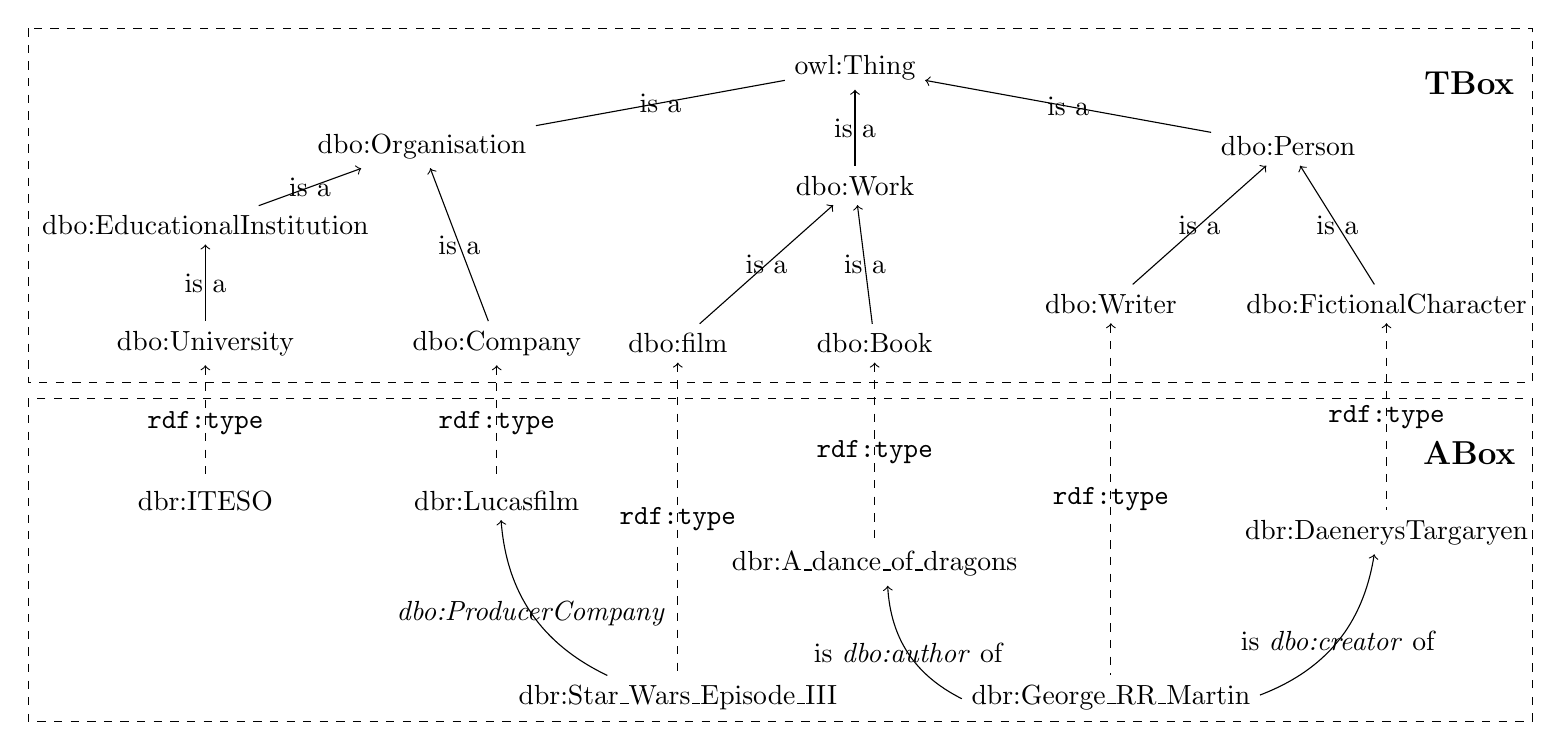
\begin{tikzpicture}

  \node {owl:Thing}[sibling distance = 5.5cm, level distance = 1cm]
    child { node {dbo:Organisation} 
        child { node {dbo:EducationalInstitution} 
            child { node [yshift = -0.5cm]{dbo:University}
            child { node [yshift = -1cm] {dbr:ITESO}
            edge from parent [<-, dashed] node {\texttt{rdf:type}}}
            edge from parent [<-] node {is a}}
        edge from parent [<-] node {is a}}
        child { node [xshift = -1.8cm, yshift = -1.5cm] {dbo:Company} edge from parent
            child {node [yshift = -1cm] (luc) {dbr:Lucasfilm}
            edge from parent [<-, dashed] node {\texttt{rdf:type}}
            }
            edge from parent [<-] node {is a}}
    edge from parent node {is a}}
    child { node [yshift = -.5cm] {dbo:Work}
        child { node [xshift = .5cm, yshift = -1cm] {dbo:film}
            child { node [yshift = -3.5cm] (swu) {dbr:Star\_Wars\_Episode\_III}
            edge from parent [<-, dashed] node {\texttt{rdf:type}}}
            edge from parent [<-] node {is a}}
        child { node [xshift = -2.5cm, yshift = -1cm] {dbo:Book}
            child { node [yshift = -1.8cm] (dance) {dbr:A\_dance\_of\_dragons}
            edge from parent [<-, dashed] node {\texttt{rdf:type}}}
            edge from parent [<-] node {is a}}
    edge from parent [<-] node {is a}}
    child { node {dbo:Person} 
      child { node [xshift = 0.5cm, yshift = -1cm]{dbo:Writer} 
        child { node [yshift = -4cm] (george) {dbr:George\_RR\_Martin}
        edge from parent [<-, dashed] node {\texttt{rdf:type}}}
      edge from parent [<-] node {is a}}
      child { node [xshift = -1.5cm, yshift = -1cm] {dbo:FictionalCharacter} 
        child { node [yshift = -1.9cm] (dany) {dbr:DaenerysTargaryen}
        edge from parent [<-, dashed] node {\texttt{rdf:type}}}
      edge from parent [<-] node {is a}}
      edge from parent [<-] node {is a}};
    
    % Draw edges between Rdf instances
    \begin{pgfonlayer}{background}
    \draw[bend left,->] (swu) to node {\textit{dbo:ProducerCompany}} (luc);
    \draw[bend right, ->] (george) to node {is \textit{dbo:creator} of} (dany);
    \draw[bend left, ->] (george) to node {is \textit{dbo:author} of} (dance) ;
    \end{pgfonlayer}
  
    % Draw rectangles indicating ABox and TBox
    %\draw[step=1cm,gray,very thin] (-11,-10) grid (10,1);
    %\fill[blue!40!white] (-11, 0.5) rectangle (10,-4);
    \draw[dashed] (-10.5, 0.5) rectangle (8.6, -4);
    \node at (7.8, -0.2){\textbf{\large TBox}};
    \draw[dashed] (-10.5, -4.2) rectangle (8.6, -8.3);
    \node at (7.8, -4.9) {\textbf{\large ABox}};
\end{tikzpicture}


\end{document}